\documentclass[letter,11pt]{article}
%\documentclass[letter,twoside,11pt]{article}

\usepackage[spanish,es-nodecimaldot]{babel}
\usepackage[utf8]{inputenc}

\usepackage{lmodern}
\usepackage[T1]{fontenc}
\usepackage{textcomp}

\usepackage{graphicx}
\usepackage{pstricks}

\usepackage{anysize}
\marginsize{3cm}{2cm}{2cm}{3cm}

\usepackage{amsmath}
\usepackage{array}

\usepackage{fancyhdr}
\usepackage{lastpage}
\pagestyle{fancy}
\fancyhf{}
\fancyhead[LE,RO]{Laboratorio de Física Básica I}
\fancyfoot[CO,CE]{\thepage\ de \pageref{LastPage}}

\special{papersize=215.9mm,279.4mm}

\usepackage[
    pdfauthor={Carlos Eduardo Caballero Burgoa},%
    pdftitle={Laboratorio de Física Básica I},%
    pdfsubject={Medidas directas},%
    colorlinks,%
    citecolor=black,%
    filecolor=black,%
    linkcolor=black,%
    urlcolor=black,
    breaklinks]{hyperref}
\usepackage{breakurl}

\newcommand{\blankpage}{
\newpage
\thispagestyle{empty}
\mbox{}
\newpage
}

\renewcommand{\arraystretch}{1.2}

\begin{document}

\begin{titlepage}
\begin{center}
{\Large UNIVERSIDAD MAYOR DE SAN SIMÓN}\\
\vspace*{0.15cm}
{\large FACULTAD DE CIENCIAS Y TECNOLOGÍA}\\
\vspace*{0.10cm}
DEPARTAMENTO DE FÍSICA\\
\vspace*{3.0cm}
{\Large \textbf{LABORATORIO DE FÍSICA BÁSICA I}}\\
\vspace*{0.3cm}
{\Large \textbf{PRACTICA No. 1}}\\
\vspace*{3.5cm}
{\Large \textbf{MEDIDAS DIRECTAS}}\\
\end{center}

\vspace*{7.4cm}
\leftskip=7.95cm
\noindent
\textbf{Estudiante:}\\
Caballero Burgoa, Carlos Eduardo.\\
\newline
\textbf{Docente:}\\
Msc. Guzmán Saavedra, Rocio.\\
\newline
\textbf{Grupo:} N5.\\
\textbf{Fecha de realización:} 11 de Octubre del 2020.\\
\textbf{Fecha de entrega:} 14 de Octubre del 2020.\\

\end{titlepage}

\blankpage

\section{Objetivo}
Ejercitar la toma de datos, y la correcta presentación del resultado de la
medida.

\section{Marco teórico}
Los resultados de las medidas nunca se corresponden con los valores reales de
las magnitudes a medir, sino que, en mayor o menor extensión, son defectuosos,
es decir, están afectados de error. Las causas que motivan tales desviaciones
pueden ser debidas al observador, al aparato o incluso a las propias
características del proceso de medida.

Una medida directa es aquella, cuyo valor se consigue directamente por
comparación con la escala de un instrumento. Se pueden realizar en una sola
medición o en una serie de mediciones.

Si las fuentes de error son únicamente de carácter aleatorio, es decir, si
influyen unas veces por exceso y otras por defecto en el resultado de la medida,
puede demostrarse que el valor que más se aproxima al verdadero valor es
precisamente el valor medio. Ello es debido a que al promediar todos los
resultados, los errores por exceso tenderán a compensarse con los errores por
defecto y ello será tanto más cierto cuanto mayor sea el número de veces que se
repita la medición.

Si se realizan $n$ mediciones directas de una magnitud física, denotadas
por:

\begin{equation}
    \{x_1,x_2,x_3,\cdots,x_i,\cdots,x_n\}
\end{equation}

Para calcular el valor representativo de esta serie de mediciones, se toma la
media aritmética:

\begin{equation}
    \bar{x} = \frac{x_1+x_2+\cdots+x_n}{n} = \frac{1}{n}\sum_{i=1}^{n} x_i
\end{equation}

Para determinar el error en la medición, se hace uso de la desviación estándar,
que es una medida de dispersión usada en estadística que nos dice cuánto tienden
a alejarse los valores concretos del promedio en una distribución.

La desviación estándar ($\sigma$) es la raíz cuadrada de la varianza ($s^2$) de
la distribución de probabilidad discreta, y puede calcularse con la siguiente
formula:

\begin{equation}
    \sigma = \sqrt{s^2}
\end{equation}

Donde:

\begin{equation}
    s^2 = \frac{1}{n}\sum_{i=1}^{n} (x_i-\bar{x})^2
\end{equation}

Aunque esta fórmula es correcta, en la práctica interesa el realizar inferencias
poblacionales, por lo que en el denominador en vez de $n$, se usa $n-1$ según la
corrección de \emph{Bessel}.

\begin{equation}
    \sigma_{n-1} = \sqrt{\frac{\sum_{i=1}^{n} (x_i-\bar{x})^2}{(n-1)}}
\end{equation}

El error de la medida, es igual a la desviación estándar dividida por la raíz
cuadrada del número de mediciones.

\begin{equation}
    \sigma_x = \frac{\sigma_{n-1}}{\sqrt{n}}
             = \sqrt{\frac{\sum_{i=1}^{n} (x_i-\bar{x})^2}{n(n-1)}}
\end{equation}

Se define a $[(\bar{x}-\sigma_x), (\bar{x}+\sigma_x)]$ como el intervalo de
confianza en el que el valor verdadero de la medición puede encontrarse según un
porcentaje de confianza definido por el modelo de distribución de probabilidad.

Para el calculo del error $e_x$ de una serie de mediciones, es recomendable
colocar el mayor valor entre el error obtenido anteriormente $\sigma_x$ y la
precisión del instrumento de medida ($P$):

\begin{equation}
    e_x = \begin{cases}
        \sigma_x, & \mbox{si }\sigma_x > P \\
        P,        & \mbox{si }\sigma_x < P
    \end{cases}
\end{equation}

El error de la medición también debe representarse en su forma porcentual con la
siguiente formula:

\begin{equation}
    E\% = \frac{e_x}{\bar{x}}\cdot100
\end{equation}

Finalmente el resultado de las mediciones será:

\begin{equation}
    x = (\bar{x}\pm e_x)[u], E\%
\end{equation}

\section{Materiales}
\begin{itemize}
\item Distanciómetro.
\item Sonómetro.
\item Acelerómetro.
\item Luxómetro.
\end{itemize}

\section{Procedimiento}
A continuación se describen los procedimientos experimentales de medición que se
llevarán a cabo.

\subsection{Medición de distancia}
\begin{enumerate}
\item Tomar una fotografía que muestre la distancia entre el instrumento y el
objeto de medición.
\item Armar un trípode para establecer una posición fija para la medición.
\item Establecer el dato de la altura en el distanciómetro.
\item Medir 30 veces la distancia al objeto a ser medido.
\item Determinar la precisión del instrumento.
\item Calcular el valor representativo, además de los errores para cada
medición.
\end{enumerate}

\subsection{Medición de la intensidad del sonido}
\begin{enumerate}
\item Tomar una fotografía que muestre el ambiente en el cual se hará la
medición.
\item Con el sonómetro medir 30 veces la intensidad del sonido en un ambiente
por 1 minuto.
\item Registrar los valores máximo, mínimo, y promedio que el sonómetro indique.
\item Determinar la precisión del instrumento.
\item Calcular el valor representativo, además de los errores para cada
medición.
\end{enumerate}

\subsection{Medición de la gravedad}
\begin{enumerate}
\item Levantar el acelerómetro a una distancia prudencial del suelo.
\item En el instrumento, comenzar a registrar las componentes X, Y, Z de
aceleración.
\item Soltar el instrumento para que tenga un movimiento en caída libre.
\item Registrar y analizar los datos capturados, y extraer el valor de la
aceleración vertical.
\item Determinar la precisión del instrumento.
\item Calcular el valor representativo, además de los errores para cada
medición.
\item Repetir 30 veces el procedimiento.
\end{enumerate}

\subsection{Medición de la intensidad de la luz}
\begin{enumerate}
\item Armar un trípode para establecer una posición fija para la medición.
\item Con el luxómetro, medir la intensidad de luz cada hora, por 12 horas.
\item Después de cada medición, tomar una fotografía del lugar de captura.
\item Determinar la precisión del instrumento.
\item Registrar el valor de la medición y calcular el error porcentual de la
medición.
\end{enumerate}

\section{Tablas de datos y resultados}

\subsection{Medición de distancia}

Medición de la longitud de la habitación que se muestra en la figura
\ref{distancia}, dado que la altura desde la cual se hace la medición es de
130[cm], la perspectiva de la aplicación de medición puede verse en la figura
\ref{medida}.

\begin{description}
\item[Instrumento utilizado:] Distanciómetro.
\item[Precisión del instrumento:] $0.01 [m]$
\end{description}

\begin{figure}
\centering
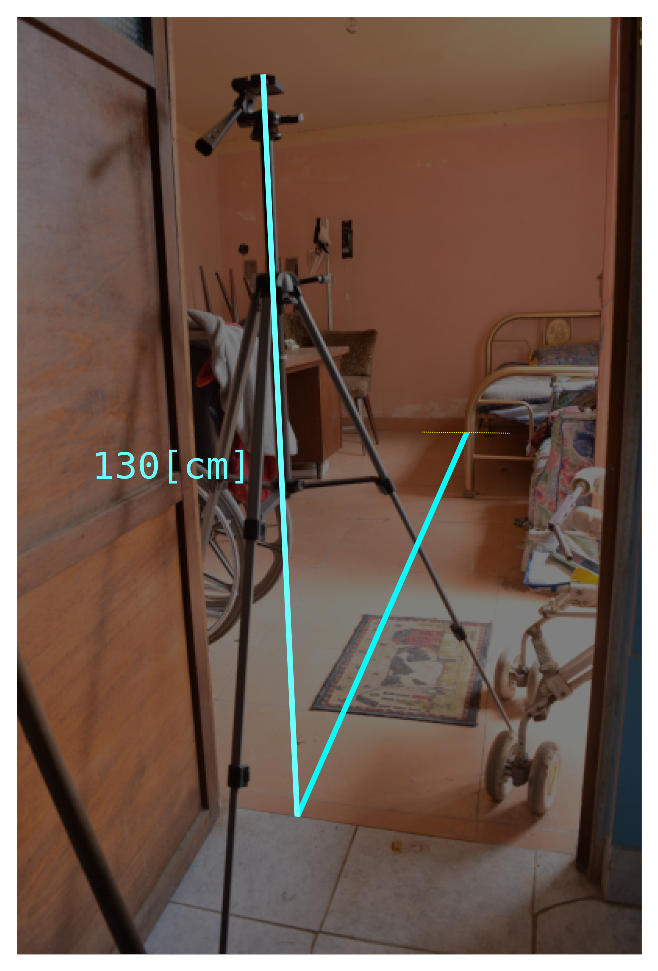
\includegraphics[width=0.45\textwidth]{eps/1.1.distancia.eps}
\caption{Longitud de la habitación}
\label{distancia}
\end{figure}

\begin{figure}
\centering
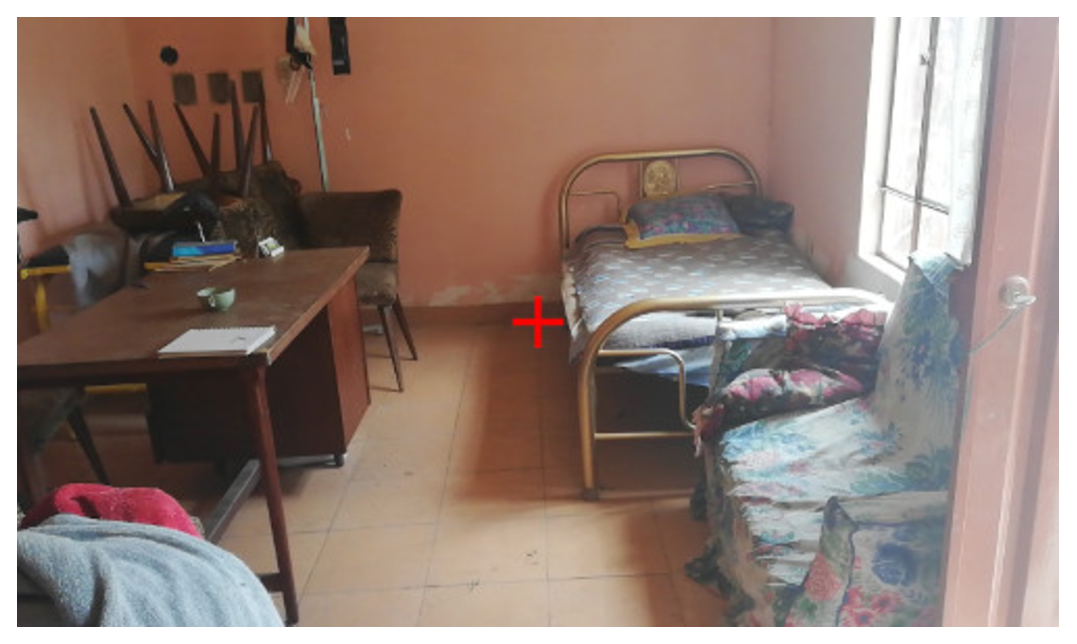
\includegraphics[width=0.75\textwidth]{eps/1.1.medida.eps}
\caption{Vista de la aplicación de medición}
\label{medida}
\end{figure}

\subsubsection{Datos obtenidos}

\begin{tabular}{|c|>{\centering}m{3.3cm}<{\centering}|}
\hline
$i$ & $x [m]$ \tabularnewline \hline
 1 & 3.99 \tabularnewline \hline
 2 & 3.90 \tabularnewline \hline
 3 & 3.86 \tabularnewline \hline
 4 & 4.02 \tabularnewline \hline
 5 & 3.90 \tabularnewline \hline
 6 & 3.96 \tabularnewline \hline
 7 & 3.86 \tabularnewline \hline
 8 & 4.09 \tabularnewline \hline
 9 & 4.07 \tabularnewline \hline
10 & 4.02 \tabularnewline \hline
11 & 3.99 \tabularnewline \hline
12 & 3.91 \tabularnewline \hline
13 & 3.95 \tabularnewline \hline
14 & 3.97 \tabularnewline \hline
15 & 3.90 \tabularnewline \hline
16 & 3.93 \tabularnewline \hline
17 & 3.88 \tabularnewline \hline
18 & 4.04 \tabularnewline \hline
19 & 3.97 \tabularnewline \hline
20 & 3.90 \tabularnewline \hline
21 & 3.84 \tabularnewline \hline
22 & 4.11 \tabularnewline \hline
23 & 3.81 \tabularnewline \hline
24 & 4.04 \tabularnewline \hline
25 & 3.97 \tabularnewline \hline
26 & 4.07 \tabularnewline \hline
27 & 3.92 \tabularnewline \hline
28 & 3.87 \tabularnewline \hline
29 & 4.00 \tabularnewline \hline
30 & 3.85 \tabularnewline \hline
$n = 30$ & $\sum{x_i} = 118.59$ \tabularnewline \hline
\end{tabular}
\quad
\begin{tabular}{|c|>{\centering}m{2.7cm}<{\centering}
                  |>{\centering}m{4.2cm}<{\centering}|}
\hline
$i$ & $x_i - \bar{x}$ & $(x_i - \bar{x})^2$ \tabularnewline \hline
 1 &  0.0370 & 0.0014 \tabularnewline \hline
 2 & -0.0530 & 0.0028 \tabularnewline \hline
 3 & -0.0930 & 0.0086 \tabularnewline \hline
 4 &  0.0670 & 0.0045 \tabularnewline \hline
 5 & -0.0530 & 0.0028 \tabularnewline \hline
 6 &  0.0070 & 0.0000 \tabularnewline \hline
 7 & -0.0930 & 0.0086 \tabularnewline \hline
 8 &  0.1370 & 0.0188 \tabularnewline \hline
 9 &  0.1170 & 0.0137 \tabularnewline \hline
10 &  0.0670 & 0.0045 \tabularnewline \hline
11 &  0.0370 & 0.0014 \tabularnewline \hline
12 & -0.0430 & 0.0018 \tabularnewline \hline
13 & -0.0030 & 0.0000 \tabularnewline \hline
14 &  0.0170 & 0.0003 \tabularnewline \hline
15 & -0.0530 & 0.0028 \tabularnewline \hline
16 & -0.0230 & 0.0005 \tabularnewline \hline
17 & -0.0730 & 0.0053 \tabularnewline \hline
18 &  0.0870 & 0.0076 \tabularnewline \hline
19 &  0.0170 & 0.0003 \tabularnewline \hline
20 & -0.0530 & 0.0028 \tabularnewline \hline
21 & -0.1130 & 0.0128 \tabularnewline \hline
22 &  0.1570 & 0.0246 \tabularnewline \hline
23 & -0.1430 & 0.0204 \tabularnewline \hline
24 &  0.0870 & 0.0076 \tabularnewline \hline
25 &  0.0170 & 0.0003 \tabularnewline \hline
26 &  0.1170 & 0.0137 \tabularnewline \hline
27 & -0.0330 & 0.0011 \tabularnewline \hline
28 & -0.0830 & 0.0069 \tabularnewline \hline
29 &  0.0470 & 0.0022 \tabularnewline \hline
30 & -0.1030 & 0.0106 \tabularnewline \hline
& & $\sum{(x_i - \bar{x})^2} = 0.1888$ \tabularnewline \hline
\end{tabular}

\vspace*{0.6cm}
\begin{tabular}{|c|>{\centering}m{4.04cm}<{\centering}|}
\hline
 $\bar{x}$ & 3.9530 \tabularnewline \hline
$\sigma_x$ & 0.0147 \tabularnewline \hline
       $P$ & 0.0100 \tabularnewline \hline
     $e_x$ & 0.0147 \tabularnewline \hline
\end{tabular}
\quad
\begin{tabular}{|c|>{\centering}m{7.52cm}<{\centering}|}
\hline
\multicolumn{2}{|c|}{\textbf{Resultado de la medición}} \\ \hline
$d$ & $(3.95\pm0.01)[m], 0.37\%$ \tabularnewline \hline
\end{tabular}

\subsubsection{Memoria de calculo}

\footnotesize
\begin{verbatim}
% practica101.m
% medicion de distancia
x = [3.99 3.90 3.86 4.02 3.90 3.96 3.86 4.09 4.07 4.02 ...
     3.99 3.91 3.95 3.97 3.90 3.93 3.88 4.04 3.97 3.90 ...
     3.84 4.11 3.81 4.04 3.97 4.07 3.92 3.87 4.00 3.85]

% tamano de la muestra
n = length(x)
% sumatoria
S = sum(x)
% promedio
m = mean(x)
% calculo de las discrepancias
d = x - m
% calculo de las discrepancias al cuadrado
d2 = d.*d
% sumatoria de las discrepancias al cuadrado
S2 = sum(d2)
% calculo del error
s = sqrt(S2 / (n * (n - 1)))
% precision del instrumento
P = 0.01
% calculo del error
e = max(s, P)
% calculo del error porcentual
E = (e / m) * 100

salida del programa
===================
>> practica101

x =
  Columns 1 through 14
    3.9900    3.9000    3.8600    4.0200    3.9000    3.9600    3.8600
    4.0900    4.0700    4.0200    3.9900    3.9100    3.9500    3.9700

  Columns 15 through 28
    3.9000    3.9300    3.8800    4.0400    3.9700    3.9000    3.8400
    4.1100    3.8100    4.0400    3.9700    4.0700    3.9200    3.8700

  Columns 29 through 30
    4.0000    3.8500

n = 30
S = 118.5900
m = 3.9530

d =
  Columns 1 through 14
    0.0370   -0.0530   -0.0930    0.0670   -0.0530    0.0070   -0.0930
    0.1370    0.1170    0.0670    0.0370   -0.0430   -0.0030    0.0170

  Columns 15 through 28
   -0.0530   -0.0230   -0.0730    0.0870    0.0170   -0.0530   -0.1130
    0.1570   -0.1430    0.0870    0.0170    0.1170   -0.0330   -0.0830

  Columns 29 through 30
    0.0470   -0.1030

d2 =
  Columns 1 through 14
    0.0014    0.0028    0.0086    0.0045    0.0028    0.0000    0.0086
    0.0188    0.0137    0.0045    0.0014    0.0018    0.0000    0.0003

  Columns 15 through 28
    0.0028    0.0005    0.0053    0.0076    0.0003    0.0028    0.0128
    0.0246    0.0204    0.0076    0.0003    0.0137    0.0011    0.0069

  Columns 29 through 30
    0.0022    0.0106

S2 = 0.1888
s = 0.0147
P = 0.0100
e = 0.0147
E = 0.3727
\end{verbatim}
\normalsize

\subsection{Medición de la intensidad de sonido}

Medición de la intensidad de sonido de la habitación que se muestra en la figura
\ref{sonometro}.

\begin{description}
\item[Instrumento utilizado:] Sonómetro.
\item[Precisión del instrumento:] $0.1 [dB]$
\end{description}

\begin{figure}
\centering
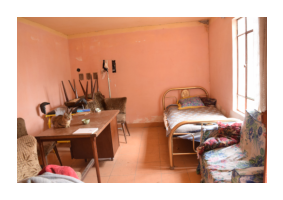
\includegraphics[width=0.75\textwidth]{eps/1.2.sonometro.eps}
\caption{Vista de la habitación a medir}
\label{sonometro}
\end{figure}

\subsubsection{Datos obtenidos (valor máximo)}

\begin{tabular}{|c|>{\centering}m{3.3cm}<{\centering}|}
\hline
$i$ & $x_{max} [dB]$ \tabularnewline \hline
 1 & 54.4 \tabularnewline \hline
 2 & 63.7 \tabularnewline \hline
 3 & 65.1 \tabularnewline \hline
 4 & 49.0 \tabularnewline \hline
 5 & 58.1 \tabularnewline \hline
 6 & 64.0 \tabularnewline \hline
 7 & 67.1 \tabularnewline \hline
 8 & 72.2 \tabularnewline \hline
 9 & 47.7 \tabularnewline \hline
10 & 48.1 \tabularnewline \hline
11 & 60.9 \tabularnewline \hline
12 & 43.6 \tabularnewline \hline
13 & 72.6 \tabularnewline \hline
14 & 61.1 \tabularnewline \hline
15 & 64.9 \tabularnewline \hline
16 & 58.6 \tabularnewline \hline
17 & 64.5 \tabularnewline \hline
18 & 59.4 \tabularnewline \hline
19 & 69.1 \tabularnewline \hline
20 & 64.2 \tabularnewline \hline
21 & 69.1 \tabularnewline \hline
22 & 58.3 \tabularnewline \hline
23 & 67.7 \tabularnewline \hline
24 & 68.4 \tabularnewline \hline
25 & 56.8 \tabularnewline \hline
26 & 57.7 \tabularnewline \hline
27 & 63.7 \tabularnewline \hline
28 & 67.2 \tabularnewline \hline
29 & 70.8 \tabularnewline \hline
30 & 57.6 \tabularnewline \hline
$n = 30$ & $\sum{x_i} = 1845.6$ \tabularnewline \hline
\end{tabular}
\quad
\begin{tabular}{|c|>{\centering}m{2.7cm}<{\centering}
                  |>{\centering}m{4.2cm}<{\centering}|}
\hline
$i$ & $x_i - \bar{x}$ & $(x_i - \bar{x})^2$ \tabularnewline \hline
 1 &  -7.1200 &  50.6944 \tabularnewline \hline
 2 &   2.1800 &   4.7524 \tabularnewline \hline
 3 &   3.5800 &  12.8164 \tabularnewline \hline
 4 & -12.5200 & 156.7504 \tabularnewline \hline
 5 &  -3.4200 &  11.6964 \tabularnewline \hline
 6 &   2.4800 &   6.1504 \tabularnewline \hline
 7 &   5.5800 &  31.1364 \tabularnewline \hline
 8 &  10.6800 & 114.0624 \tabularnewline \hline
 9 & -13.8200 & 190.9924 \tabularnewline \hline
10 & -13.4200 & 180.0964 \tabularnewline \hline
11 &  -0.6200 &   0.3844 \tabularnewline \hline
12 & -17.9200 & 321.1264 \tabularnewline \hline
13 &  11.0800 & 122.7664 \tabularnewline \hline
14 &  -0.4200 &   0.1764 \tabularnewline \hline
15 &   3.3800 &  11.4244 \tabularnewline \hline
16 &  -2.9200 &   8.5264 \tabularnewline \hline
17 &   2.9800 &   8.8804 \tabularnewline \hline
18 &  -2.1200 &   4.4944 \tabularnewline \hline
19 &   7.5800 &  57.4564 \tabularnewline \hline
20 &   2.6800 &   7.1824 \tabularnewline \hline
21 &   7.5800 &  57.4564 \tabularnewline \hline
22 &  -3.2200 &  10.3684 \tabularnewline \hline
23 &   6.1800 &  38.1924 \tabularnewline \hline
24 &   6.8800 &  47.3344 \tabularnewline \hline
25 &  -4.7200 &  22.2784 \tabularnewline \hline
26 &  -3.8200 &  14.5924 \tabularnewline \hline
27 &   2.1800 &   4.7524 \tabularnewline \hline
28 &   5.6800 &  32.2624 \tabularnewline \hline
29 &   9.2800 &  86.1184 \tabularnewline \hline
30 &  -3.9200 &  15.3664 \tabularnewline \hline
& & $\sum{(x_i - \bar{x})^2} = 1630.3$ \tabularnewline \hline
\end{tabular}

\vspace*{0.5cm}
\begin{tabular}{|c|>{\centering}m{4.04cm}<{\centering}|}
\hline
 $\bar{x}$ & 61.5200 \tabularnewline \hline
$\sigma_x$ &  1.3689 \tabularnewline \hline
       $P$ &  0.1000 \tabularnewline \hline
     $e_x$ &  1.3689 \tabularnewline \hline
\end{tabular}
\quad
\begin{tabular}{|c|>{\centering}m{6.92cm}<{\centering}|}
\hline
\multicolumn{2}{|c|}{\textbf{Resultado de la medición}} \\ \hline
$s_{max}$ & $(61.5\pm1.4)[dB], 2.23\%$ \tabularnewline \hline
\end{tabular}

\subsubsection{Memoria de calculo (valor máximo)}

\footnotesize
\begin{verbatim}
% practica102.m
% medicion del maximo de la intensidad del sonido
x = [54.4 63.7 65.1 49.0 58.1 64.0 67.1 72.2 47.7 48.1 ...
     60.9 43.6 72.6 61.1 64.9 58.6 64.5 59.4 69.1 64.2 ...
     69.1 58.3 67.7 68.4 56.8 57.7 63.7 67.2 70.8 57.6]

% tamano de la muestra
n = length(x)
% sumatoria
S = sum(x)
% promedio
m = mean(x)
% calculo de las discrepancias
d = x - m
% calculo de las discrepancias al cuadrado
d2 = d.*d
% sumatoria de las discrepancias al cuadrado
S2 = sum(d2)
% calculo del error
s = sqrt(S2 / (n * (n - 1)))
% precision del instrumento
P = 0.1
% calculo del error
e = max(s, P)
% calculo del error porcentual
E = (e / m) * 100

salida del programa
===================
>> practica102

x =
  Columns 1 through 14
   54.4000   63.7000   65.1000   49.0000   58.1000   64.0000   67.1000
   72.2000   47.7000   48.1000   60.9000   43.6000   72.6000   61.1000

  Columns 15 through 28
   64.9000   58.6000   64.5000   59.4000   69.1000   64.2000   69.1000
   58.3000   67.7000   68.4000   56.8000   57.7000   63.7000   67.2000

  Columns 29 through 30
   70.8000   57.6000

n = 30
S = 1.8456e+03
m = 61.5200

d =
  Columns 1 through 14
   -7.1200    2.1800    3.5800  -12.5200   -3.4200    2.4800    5.5800
   10.6800  -13.8200  -13.4200   -0.6200  -17.9200   11.0800   -0.4200

  Columns 15 through 28
    3.3800   -2.9200    2.9800   -2.1200    7.5800    2.6800    7.5800
   -3.2200    6.1800    6.8800   -4.7200   -3.8200    2.1800    5.6800

  Columns 29 through 30
    9.2800   -3.9200

d2 =
  Columns 1 through 14
    50.6944    4.7524   12.8164  156.7504   11.6964    6.1504   31.1364
   114.0624  190.9924  180.0964    0.3844  321.1264  122.7664    0.1764

  Columns 15 through 28
   11.4244    8.5264    8.8804    4.4944   57.4564    7.1824   57.4564
   10.3684   38.1924   47.3344   22.2784   14.5924    4.7524   32.2624

  Columns 29 through 30
   86.1184   15.3664

S2 = 1.6303e+03
s = 1.3689
P = 0.1000
e = 1.3689
E = 2.2251
\end{verbatim}
\normalsize

\subsubsection{Datos obtenidos (valor mínimo)}

\begin{tabular}{|c|>{\centering}m{3.3cm}<{\centering}|}
\hline
$i$ & $x_{min} [dB]$ \tabularnewline \hline
 1 & 26.8 \tabularnewline \hline
 2 & 27.8 \tabularnewline \hline
 3 & 27.3 \tabularnewline \hline
 4 & 25.3 \tabularnewline \hline
 5 & 24.7 \tabularnewline \hline
 6 & 25.5 \tabularnewline \hline
 7 & 27.1 \tabularnewline \hline
 8 & 30.4 \tabularnewline \hline
 9 & 25.0 \tabularnewline \hline
10 & 25.0 \tabularnewline \hline
11 & 27.5 \tabularnewline \hline
12 & 24.0 \tabularnewline \hline
13 & 31.7 \tabularnewline \hline
14 & 26.8 \tabularnewline \hline
15 & 27.6 \tabularnewline \hline
16 & 25.6 \tabularnewline \hline
17 & 27.1 \tabularnewline \hline
18 & 25.2 \tabularnewline \hline
19 & 29.8 \tabularnewline \hline
20 & 26.3 \tabularnewline \hline
21 & 29.0 \tabularnewline \hline
22 & 28.0 \tabularnewline \hline
23 & 28.6 \tabularnewline \hline
24 & 31.1 \tabularnewline \hline
25 & 28.7 \tabularnewline \hline
26 & 30.7 \tabularnewline \hline
27 & 28.1 \tabularnewline \hline
28 & 30.0 \tabularnewline \hline
29 & 32.3 \tabularnewline \hline
30 & 25.5 \tabularnewline \hline
$n = 30$ & $\sum{x_i} = 828.5$ \tabularnewline \hline
\end{tabular}
\quad
\begin{tabular}{|c|>{\centering}m{2.7cm}<{\centering}
                  |>{\centering}m{4.2cm}<{\centering}|}
\hline
$i$ & $x_i - \bar{x}$ & $(x_i - \bar{x})^2$ \tabularnewline \hline
 1 & -0.8167 &  0.6669 \tabularnewline \hline
 2 &  0.1833 &  0.0336 \tabularnewline \hline
 3 & -0.3167 &  0.1003 \tabularnewline \hline
 4 & -2.3167 &  5.3669 \tabularnewline \hline
 5 & -2.9167 &  8.5069 \tabularnewline \hline
 6 & -2.1167 &  4.4803 \tabularnewline \hline
 7 & -0.5167 &  0.2669 \tabularnewline \hline
 8 &  2.7833 &  7.7469 \tabularnewline \hline
 9 & -2.6167 &  6.8469 \tabularnewline \hline
10 & -2.6167 &  6.8469 \tabularnewline \hline
11 & -0.1167 &  0.0136 \tabularnewline \hline
12 & -3.6167 & 13.0803 \tabularnewline \hline
13 &  4.0833 & 16.6736 \tabularnewline \hline
14 & -0.8167 &  0.6669 \tabularnewline \hline
15 & -0.0167 &  0.0003 \tabularnewline \hline
16 & -2.0167 &  4.0669 \tabularnewline \hline
17 & -0.5167 &  0.2669 \tabularnewline \hline
18 & -2.4167 &  5.8403 \tabularnewline \hline
19 &  2.1833 &  4.7669 \tabularnewline \hline
20 & -1.3167 &  1.7336 \tabularnewline \hline
21 &  1.3833 &  1.9136 \tabularnewline \hline
22 &  0.3833 &  0.1469 \tabularnewline \hline
23 &  0.9833 &  0.9669 \tabularnewline \hline
24 &  3.4833 & 12.1336 \tabularnewline \hline
25 &  1.0833 &  1.1736 \tabularnewline \hline
26 &  3.0833 &  9.5069 \tabularnewline \hline
27 &  0.4833 &  0.2336 \tabularnewline \hline
28 &  2.3833 &  5.6803 \tabularnewline \hline
29 &  4.6833 & 21.9336 \tabularnewline \hline
30 & -2.1167 &  4.4803 \tabularnewline \hline
& & $\sum{(x_i - \bar{x})^2} = 146.1417$ \tabularnewline \hline
\end{tabular}

\vspace*{0.5cm}
\begin{tabular}{|c|>{\centering}m{4.04cm}<{\centering}|}
\hline
 $\bar{x}$ & 27.6167 \tabularnewline \hline
$\sigma_x$ &  0.4099 \tabularnewline \hline
       $P$ &  0.1000 \tabularnewline \hline
     $e_x$ &  0.4099 \tabularnewline \hline
\end{tabular}
\quad
\begin{tabular}{|c|>{\centering}m{6.92cm}<{\centering}|}
\hline
\multicolumn{2}{|c|}{\textbf{Resultado de la medición}} \\ \hline
$s_{min}$ & $(27.6\pm0.4)[dB], 1.48\%$ \tabularnewline \hline
\end{tabular}

\subsubsection{Memoria de calculo (valor mínimo)}

\footnotesize
\begin{verbatim}
% practica103.m
% medicion del minimo de la intensidad del sonido
x = [26.8 27.8 27.3 25.3 24.7 25.5 27.1 30.4 25.0 25.0 ...
     27.5 24.0 31.7 26.8 27.6 25.6 27.1 25.2 29.8 26.3 ...
     29.0 28.0 28.6 31.1 28.7 30.7 28.1 30.0 32.3 25.5]

% tamano de la muestra
n = length(x)
% sumatoria
S = sum(x)
% promedio
m = mean(x)
% calculo de las discrepancias
d = x - m
% calculo de las discrepancias al cuadrado
d2 = d.*d
% sumatoria de las discrepancias al cuadrado
S2 = sum(d2)
% calculo del error
s = sqrt(S2 / (n * (n - 1)))
% precision del instrumento
P = 0.1
% calculo del error
e = max(s, P)
% calculo del error porcentual
E = (e / m) * 100

salida del programa
===================
>> practica103

x =
  Columns 1 through 14
   26.8000   27.8000   27.3000   25.3000   24.7000   25.5000   27.1000
   30.4000   25.0000   25.0000   27.5000   24.0000   31.7000   26.8000

  Columns 15 through 28
   27.6000   25.6000   27.1000   25.2000   29.8000   26.3000   29.0000
   28.0000   28.6000   31.1000   28.7000   30.7000   28.1000   30.0000

  Columns 29 through 30
   32.3000   25.5000

n = 30
S = 828.5000
m = 27.6167

d =
  Columns 1 through 14
   -0.8167    0.1833   -0.3167   -2.3167   -2.9167   -2.1167   -0.5167
    2.7833   -2.6167   -2.6167   -0.1167   -3.6167    4.0833   -0.8167

  Columns 15 through 28
   -0.0167   -2.0167   -0.5167   -2.4167    2.1833   -1.3167    1.3833
    0.3833    0.9833    3.4833    1.0833    3.0833    0.4833    2.3833

  Columns 29 through 30
    4.6833   -2.1167

d2 =
  Columns 1 through 14
    0.6669    0.0336    0.1003    5.3669    8.5069    4.4803    0.2669
    7.7469    6.8469    6.8469    0.0136   13.0803   16.6736    0.6669

  Columns 15 through 28
    0.0003    4.0669    0.2669    5.8403    4.7669    1.7336    1.9136
    0.1469    0.9669   12.1336    1.1736    9.5069    0.2336    5.6803

  Columns 29 through 30
   21.9336    4.4803

S2 = 146.1417
s = 0.4099
P = 0.1000
e = 0.4099
E = 1.4841
\end{verbatim}
\normalsize

\subsubsection{Datos obtenidos (valor promedio)}

\begin{tabular}{|c|>{\centering}m{3.3cm}<{\centering}|}
\hline
$i$ & $x_{avg} [dB]$ \tabularnewline \hline
 1 & 40.1 \tabularnewline \hline
 2 & 38.8 \tabularnewline \hline
 3 & 41.9 \tabularnewline \hline
 4 & 35.1 \tabularnewline \hline
 5 & 37.9 \tabularnewline \hline
 6 & 40.0 \tabularnewline \hline
 7 & 44.3 \tabularnewline \hline
 8 & 50.2 \tabularnewline \hline
 9 & 35.8 \tabularnewline \hline
10 & 34.7 \tabularnewline \hline
11 & 40.7 \tabularnewline \hline
12 & 33.8 \tabularnewline \hline
13 & 52.5 \tabularnewline \hline
14 & 40.5 \tabularnewline \hline
15 & 41.5 \tabularnewline \hline
16 & 40.9 \tabularnewline \hline
17 & 43.6 \tabularnewline \hline
18 & 39.2 \tabularnewline \hline
19 & 45.7 \tabularnewline \hline
20 & 45.6 \tabularnewline \hline
21 & 45.2 \tabularnewline \hline
22 & 41.6 \tabularnewline \hline
23 & 45.7 \tabularnewline \hline
24 & 48.5 \tabularnewline \hline
25 & 41.8 \tabularnewline \hline
26 & 43.2 \tabularnewline \hline
27 & 42.7 \tabularnewline \hline
28 & 45.6 \tabularnewline \hline
29 & 49.8 \tabularnewline \hline
30 & 35.9 \tabularnewline \hline
$n = 30$ & $\sum{x_i} = 1262.8 $ \tabularnewline \hline
\end{tabular}
\quad
\begin{tabular}{|c|>{\centering}m{2.7cm}<{\centering}
                  |>{\centering}m{4.2cm}<{\centering}|}
\hline
$i$ & $x_i - \bar{x}$ & $(x_i - \bar{x})^2$ \tabularnewline \hline
 1 & -1.9933 &   3.9734 \tabularnewline \hline
 2 & -3.2933 &  10.8460 \tabularnewline \hline
 3 & -0.1933 &   0.0374 \tabularnewline \hline
 4 & -6.9933 &  48.9067 \tabularnewline \hline
 5 & -4.1933 &  17.5840 \tabularnewline \hline
 6 & -2.0933 &   4.3820 \tabularnewline \hline
 7 &  2.2067 &   4.8694 \tabularnewline \hline
 8 &  8.1067 &  65.7180 \tabularnewline \hline
 9 & -6.2933 &  39.6060 \tabularnewline \hline
10 & -7.3933 &  54.6614 \tabularnewline \hline
11 & -1.3933 &   1.9414 \tabularnewline \hline
12 & -8.2933 &  68.7794 \tabularnewline \hline
13 & 10.4067 & 108.2987 \tabularnewline \hline
14 & -1.5933 &   2.5387 \tabularnewline \hline
15 & -0.5933 &   0.3520 \tabularnewline \hline
16 & -1.1933 &   1.4240 \tabularnewline \hline
17 &  1.5067 &   2.2700 \tabularnewline \hline
18 & -2.8933 &   8.3714 \tabularnewline \hline
19 &  3.6067 &  13.0080 \tabularnewline \hline
20 &  3.5067 &  12.2967 \tabularnewline \hline
21 &  3.1067 &   9.6514 \tabularnewline \hline
22 & -0.4933 &   0.2434 \tabularnewline \hline
23 &  3.6067 &  13.0080 \tabularnewline \hline
24 &  6.4067 &  41.0454 \tabularnewline \hline
25 & -0.2933 &   0.0860 \tabularnewline \hline
26 &  1.1067 &   1.2247 \tabularnewline \hline
27 &  0.6067 &   0.3680 \tabularnewline \hline
28 &  3.5067 &  12.2967 \tabularnewline \hline
29 &  7.7067 &  59.3927 \tabularnewline \hline
30 & -6.1933 &  38.3574 \tabularnewline \hline
& & $\sum{(x_i - \bar{x})^2} = 645.5387$ \tabularnewline \hline
\end{tabular}

\vspace*{0.5cm}
\begin{tabular}{|c|>{\centering}m{4.04cm}<{\centering}|}
\hline
 $\bar{x}$ & 42.0933 \tabularnewline \hline
$\sigma_x$ & 0.8614 \tabularnewline \hline
       $P$ & 0.1000 \tabularnewline \hline
     $e_x$ & 0.8614 \tabularnewline \hline
\end{tabular}
\quad
\begin{tabular}{|c|>{\centering}m{7.04cm}<{\centering}|}
\hline
\multicolumn{2}{|c|}{\textbf{Resultado de la medición}} \\ \hline
$s_{avg}$ & $(42.1\pm0.9)[dB], 2.05\%$ \tabularnewline \hline
\end{tabular}

\subsubsection{Memoria de calculo (valor promedio)}

\footnotesize
\begin{verbatim}
% practica104.m
% medicion del promedio de la intensidad del sonido
x = [40.1 38.8 41.9 35.1 37.9 40.0 44.3 50.2 35.8 34.7 ...
     40.7 33.8 52.5 40.5 41.5 40.9 43.6 39.2 45.7 45.6 ...
     45.2 41.6 45.7 48.5 41.8 43.2 42.7 45.6 49.8 35.9]

% tamano de la muestra
n = length(x)
% sumatoria
S = sum(x)
% promedio
m = mean(x)
% calculo de las discrepancias
d = x - m
% calculo de las discrepancias al cuadrado
d2 = d.*d
% sumatoria de las discrepancias al cuadrado
S2 = sum(d2)
% calculo del error
s = sqrt(S2 / (n * (n - 1)))
% precision del instrumento
P = 0.1
% calculo del error
e = max(s, P)
% calculo del error porcentual
E = (e / m) * 100

salida del programa
===================
>> practica104

x =
  Columns 1 through 14
   40.1000   38.8000   41.9000   35.1000   37.9000   40.0000   44.3000
   50.2000   35.8000   34.7000   40.7000   33.8000   52.5000   40.5000

  Columns 15 through 28
   41.5000   40.9000   43.6000   39.2000   45.7000   45.6000   45.2000
   41.6000   45.7000   48.5000   41.8000   43.2000   42.7000   45.6000

  Columns 29 through 30
   49.8000   35.9000

n = 30
S = 1.2628e+03
m = 42.0933

d =
  Columns 1 through 14
   -1.9933   -3.2933   -0.1933   -6.9933   -4.1933   -2.0933    2.2067
    8.1067   -6.2933   -7.3933   -1.3933   -8.2933   10.4067   -1.5933

  Columns 15 through 28
   -0.5933   -1.1933    1.5067   -2.8933    3.6067    3.5067    3.1067
   -0.4933    3.6067    6.4067   -0.2933    1.1067    0.6067    3.5067

  Columns 29 through 30
    7.7067   -6.1933

d2 =
  Columns 1 through 14
     3.9734   10.8460    0.0374   48.9067   17.5840    4.3820    4.8694
    65.7180   39.6060   54.6614    1.9414   68.7794  108.2987    2.5387

  Columns 15 through 28
    0.3520    1.4240    2.2700    8.3714   13.0080   12.2967    9.6514
    0.2434   13.0080   41.0454    0.0860    1.2247    0.3680   12.2967

  Columns 29 through 30
   59.3927   38.3574

S2 = 645.5387
s = 0.8614
P = 0.1000
e = 0.8614
E = 2.0464
\end{verbatim}
\normalsize

\subsection{Medición de la gravedad}

\begin{description}
\item[Instrumento utilizado:] Acelerómetro.
\item[Precisión del instrumento:] $0.0001 [m/s^2]$
\end{description}

\begin{tabular}{|c|>{\centering}m{3.3cm}<{\centering}|}
\hline
$i$ & $x [m/s^2]$ \tabularnewline \hline
 1 & 9.8171 \tabularnewline \hline
 2 & 9.7927 \tabularnewline \hline
 3 & 9.8116 \tabularnewline \hline
 4 & 9.7834 \tabularnewline \hline
 5 & 9.7835 \tabularnewline \hline
 6 & 9.8316 \tabularnewline \hline
 7 & 9.7927 \tabularnewline \hline
 8 & 9.8304 \tabularnewline \hline
 9 & 9.7969 \tabularnewline \hline
10 & 9.7678 \tabularnewline \hline
11 & 9.7338 \tabularnewline \hline
12 & 9.8094 \tabularnewline \hline
13 & 9.9700 \tabularnewline \hline
14 & 9.7969 \tabularnewline \hline
15 & 9.5951 \tabularnewline \hline
16 & 9.7448 \tabularnewline \hline
17 & 9.7952 \tabularnewline \hline
18 & 9.7913 \tabularnewline \hline
19 & 9.6635 \tabularnewline \hline
20 & 9.8145 \tabularnewline \hline
21 & 9.7254 \tabularnewline \hline
22 & 9.7533 \tabularnewline \hline
23 & 9.7943 \tabularnewline \hline
24 & 9.7682 \tabularnewline \hline
25 & 9.6722 \tabularnewline \hline
26 & 9.7603 \tabularnewline \hline
27 & 9.8135 \tabularnewline \hline
28 & 9.7913 \tabularnewline \hline
29 & 9.7124 \tabularnewline \hline
30 & 9.7172 \tabularnewline \hline
$n = 30$ & $\sum{x_i} = 293.2303 $ \tabularnewline \hline
\end{tabular}
\quad
\begin{tabular}{|c|>{\centering}m{2.7cm}<{\centering}
                  |>{\centering}m{4.2cm}<{\centering}|}
\hline
$i$ & $x_i - \bar{x}$ & $(x_i - \bar{x})^2$ \tabularnewline \hline
 1 &  0.0428 & 0.0018 \tabularnewline \hline
 2 &  0.0184 & 0.0003 \tabularnewline \hline
 3 &  0.0373 & 0.0014 \tabularnewline \hline
 4 &  0.0091 & 0.0001 \tabularnewline \hline
 5 &  0.0092 & 0.0001 \tabularnewline \hline
 6 &  0.0573 & 0.0033 \tabularnewline \hline
 7 &  0.0184 & 0.0003 \tabularnewline \hline
 8 &  0.0561 & 0.0031 \tabularnewline \hline
 9 &  0.0226 & 0.0005 \tabularnewline \hline
10 & -0.0065 & 0.0000 \tabularnewline \hline
11 & -0.0405 & 0.0016 \tabularnewline \hline
12 &  0.0351 & 0.0012 \tabularnewline \hline
13 &  0.1957 & 0.0383 \tabularnewline \hline
14 &  0.0226 & 0.0005 \tabularnewline \hline
15 & -0.1792 & 0.0321 \tabularnewline \hline
16 & -0.0295 & 0.0009 \tabularnewline \hline
17 &  0.0209 & 0.0004 \tabularnewline \hline
18 &  0.0170 & 0.0003 \tabularnewline \hline
19 & -0.1108 & 0.0123 \tabularnewline \hline
20 &  0.0402 & 0.0016 \tabularnewline \hline
21 & -0.0489 & 0.0024 \tabularnewline \hline
22 & -0.0210 & 0.0004 \tabularnewline \hline
23 &  0.0200 & 0.0004 \tabularnewline \hline
24 & -0.0061 & 0.0000 \tabularnewline \hline
25 & -0.1021 & 0.0104 \tabularnewline \hline
26 & -0.0140 & 0.0002 \tabularnewline \hline
27 &  0.0392 & 0.0015 \tabularnewline \hline
28 &  0.0170 & 0.0003 \tabularnewline \hline
29 & -0.0619 & 0.0038 \tabularnewline \hline
30 & -0.0571 & 0.0033 \tabularnewline \hline
& & $\sum{(x_i - \bar{x})^2} = 0.1231$ \tabularnewline \hline
\end{tabular}

\vspace*{0.5cm}
\begin{tabular}{|c|>{\centering}m{4.04cm}<{\centering}|}
\hline
 $\bar{x}$ & 9.7743 \tabularnewline \hline
$\sigma_x$ & 0.0119 \tabularnewline \hline
       $P$ & 0.0001 \tabularnewline \hline
     $e_x$ & 0.0119 \tabularnewline \hline
\end{tabular}
\quad
\begin{tabular}{|c|>{\centering}m{7.50cm}<{\centering}|}
\hline
\multicolumn{2}{|c|}{\textbf{Resultado de la medición}} \\ \hline
$g$ & $(9.8\pm0.01)[m/s^2], 0.12\%$ \tabularnewline \hline
\end{tabular}

\subsubsection{Memoria de calculo}

\footnotesize
\begin{verbatim}
% practica105.m
% medicion  de la gravedad
x = [9.8171 9.7927 9.8116 9.7834 9.7835 9.8316 9.7927 9.8304 9.7969 9.7678 ...
     9.7338 9.8094 9.9700 9.7969 9.5951 9.7448 9.7952 9.7913 9.6635 9.8145 ...
     9.7254 9.7533 9.7943 9.7682 9.6722 9.7603 9.8135 9.7913 9.7124 9.7172]

% tamano de la muestra
n = length(x)
% sumatoria
S = sum(x)
% promedio
m = mean(x)
% calculo de las discrepancias
d = x - m
% calculo de las discrepancias al cuadrado
d2 = d.*d
% sumatoria de las discrepancias al cuadrado
S2 = sum(d2)
% calculo del error
s = sqrt(S2 / (n * (n - 1)))
% precision del instrumento
P = 0.0001
% calculo del error
e = max(s, P)
% calculo del error porcentual
E = (e / m) * 100

salida del programa
===================
>> practica105

x =
  Columns 1 through 14
    9.8171    9.7927    9.8116    9.7834    9.7835    9.8316    9.7927
    9.8304    9.7969    9.7678    9.7338    9.8094    9.9700    9.7969

  Columns 15 through 28
    9.5951    9.7448    9.7952    9.7913    9.6635    9.8145    9.7254
    9.7533    9.7943    9.7682    9.6722    9.7603    9.8135    9.7913

  Columns 29 through 30
    9.7124    9.7172

n = 30
S = 293.2303
m = 9.7743

d =
  Columns 1 through 14
    0.0428    0.0184    0.0373    0.0091    0.0092    0.0573    0.0184
    0.0561    0.0226   -0.0065   -0.0405    0.0351    0.1957    0.0226

  Columns 15 through 28
   -0.1792   -0.0295    0.0209    0.0170   -0.1108    0.0402   -0.0489
   -0.0210    0.0200   -0.0061   -0.1021   -0.0140    0.0392    0.0170

  Columns 29 through 30
   -0.0619   -0.0571

d2 =
  Columns 1 through 14
    0.0018    0.0003    0.0014    0.0001    0.0001    0.0033    0.0003
    0.0031    0.0005    0.0000    0.0016    0.0012    0.0383    0.0005

  Columns 15 through 28
    0.0321    0.0009    0.0004    0.0003    0.0123    0.0016    0.0024
    0.0004    0.0004    0.0000    0.0104    0.0002    0.0015    0.0003

  Columns 29 through 30
    0.0038    0.0033

S2 = 0.1231
s = 0.0119
P = 0.0001
e = 0.0119
E = 0.1217
\end{verbatim}
\normalsize

\subsection{Medición de la intensidad de la luz}

\begin{description}
\item[Instrumento utilizado:] Luxómetro.
\item[Precisión del instrumento:] $1 [lx]$
\end{description}

\begin{tabular}{|c|c|c|}
\hline
\textbf{07:00} & \textbf{08:00} & \textbf{09:00} \tabularnewline
$L=(93\pm1)[lx], 1.07\%$ &
$L=(457\pm1)[lx], 0.22\%$ &
$L=(117\pm1)[lx], 0.85\%$ \tabularnewline

\includegraphics[width=0.293\textwidth]{eps/1.4.luxometro.07.eps} &

\includegraphics[width=0.293\textwidth]{eps/1.4.luxometro.08.eps} &

\includegraphics[width=0.293\textwidth]{eps/1.4.luxometro.09.eps}
\tabularnewline \hline
\textbf{10:00} & \textbf{11:00} & \textbf{12:00} \tabularnewline
$L=(158\pm1)[lx], 0.63\%$ &
$L=(98\pm1)[lx], 1.02\%$ &
$L=(82\pm1)[lx], 1.22\%$ \tabularnewline

\includegraphics[width=0.293\textwidth]{eps/1.4.luxometro.10.eps} &

\includegraphics[width=0.293\textwidth]{eps/1.4.luxometro.11.eps} &

\includegraphics[width=0.293\textwidth]{eps/1.4.luxometro.12.eps}
\tabularnewline \hline
\textbf{13:00} & \textbf{14:00} & \textbf{15:00} \tabularnewline
$L=(65\pm1)[lx], 1.54\%$ &
$L=(63\pm1)[lx], 1.59\%$ &
$L=(89\pm1)[lx], 1.12\%$ \tabularnewline

\includegraphics[width=0.293\textwidth]{eps/1.4.luxometro.13.eps} &

\includegraphics[width=0.293\textwidth]{eps/1.4.luxometro.14.eps} &

\includegraphics[width=0.293\textwidth]{eps/1.4.luxometro.15.eps}
\tabularnewline \hline
\textbf{16:00} & \textbf{17:00} & \textbf{18:00} \tabularnewline
$L=(34\pm1)[lx], 2.94\%$ &
$L=(9\pm1)[lx], 11.11\%$ &
$L=(3\pm1)[lx], 33.33\%$ \tabularnewline

\includegraphics[width=0.293\textwidth]{eps/1.4.luxometro.16.eps} &

\includegraphics[width=0.293\textwidth]{eps/1.4.luxometro.17.eps} &

\includegraphics[width=0.293\textwidth]{eps/1.4.luxometro.18.eps}
\tabularnewline \hline
\end{tabular}

\section{Conclusiones}
Se aprendió a medir distancias, intensidad de sonido, aceleración, y intensidad
de la luz a partir de las aplicaciones del celular. Se han obtenido medidas
directas a partir de la toma de series de medidas, y la toma de medidas únicas.

Se ha notado la importancia del manejo de la precisión en la toma de muestras,
además se ha visto que las herramientas estadísticas brindan una ayuda vital a
la tarea en laboratorio.

\subsection{Resultados obtenidos}

\begin{center}
\begin{tabular}{|c|c|}
\hline
\multicolumn{2}{|c|}{\textbf{Distanciómetro}} \\
\hline
\multicolumn{2}{|c|}{$(3.95\pm0.01)[m], 0.37\%$} \\
\hline
\multicolumn{2}{|c|}{\textbf{Sonómetro}} \\
\hline
\textbf{Máximo} & $(61.5\pm1.4)[dB], 2.23\%$ \\
\textbf{Mínimo} & $(27.6\pm0.4)[dB], 1.48\%$ \\
\textbf{Promedio} & $(42.1\pm0.9)[dB], 2.05\%$ \\
\hline
\multicolumn{2}{|c|}{\textbf{Acelerómetro}} \\
\hline
\multicolumn{2}{|c|}{$(9.8\pm0.01)[m/s^2], 0.12\%$} \\
\hline
\multicolumn{2}{|c|}{\textbf{Luxómetro}} \\
\hline
\textbf{07:00} & $( 93\pm1)[lx],  1.07\%$ \\
\textbf{08:00} & $(457\pm1)[lx],  0.22\%$ \\
\textbf{09:00} & $(117\pm1)[lx],  0.85\%$ \\
\textbf{10:00} & $(158\pm1)[lx],  0.63\%$ \\
\textbf{11:00} & $( 98\pm1)[lx],  1.02\%$ \\
\textbf{12:00} & $( 82\pm1)[lx],  1.22\%$ \\
\textbf{13:00} & $( 65\pm1)[lx],  1.54\%$ \\
\textbf{14:00} & $( 63\pm1)[lx],  1.59\%$ \\
\textbf{15:00} & $( 89\pm1)[lx],  1.12\%$ \\
\textbf{16:00} & $( 34\pm1)[lx],  2.94\%$ \\
\textbf{17:00} & $(  9\pm1)[lx], 11.11\%$ \\
\textbf{18:00} & $(  3\pm1)[lx], 33.33\%$ \\
\hline
\end{tabular}
\end{center}

\section{Referencias bibliográficas}
\begin{itemize}
\item Fisicanet \\
https://www.fisicanet.com.ar/fisica/mediciones/ap01-mediciones-errores.php
\item Desviación típica \\
https://es.wikipedia.org/wiki/Desviación\_típica
\end{itemize}

\end{document}
